\chapter{Introduction}
\label{chap1}
\textit{In this chapter, the background of soft quadruped robots and reinforcement learning approaches to its control is presented. Formulated research questions are listed together with methodologies. In addition, the limitations and delimitation to this thesis are discussed, as well as the ethics and sustainability analysis.}

\section{The Background}
In the realm of engineering, robotics emerges as a magnificent confluence of mechanical, electrical, and computer science, orchestrating a symphony of autonomous systems designed to push the boundaries of human potential and expanding efficiency\cite{billardTrendsChallengesRobot2019}. The involvement of robotic systems in our everyday lives has become increasingly commonplace, with its presence being felt across diverse fields such as manufacturing\cite{wangCurrentResearchesFuture2018}, agriculture\cite{liDevelopmentFieldEvaluation2023}, transportation\cite{zhangFindingCriticalScenarios2023}, education\cite{riedoThymioIIRobot2013} and even personal assistance\cite{openaiGPT4TechnicalReport2023}. In the domain of mobile robotics, the conventional approach to locomotion has been through the usage of wheels or tracks, making them apt for navigation on smooth surfaces\cite{liResearchMammalBionic2011}. Nonetheless, when it comes to maneuvering through unstructured and hazardous environments, such as the ones often encountered during search and rescue missions\cite{hawkesSoftRobotThat2017}, industrial production lines\cite{huDesignQuadrupedInspection2021}, or scientific research endeavors\cite{hewingLearningbasedModelPredictive2020}, legged robots, characterized by their flexible structures, have demonstrated their worth. However, recent advancements in material sciences and design have given rise to a new breed of robots known as soft robots. These robots, owing to their deformable structure, have the unique ability to mold themselves according to their surroundings, which makes them ideal for interacting with humans or fragile objects in a safe manner\cite{muralidharanSoftQuadrupedRobot2021}. This necessitates the development of advanced control strategies that can adapt to the dynamic and ever-changing morphology of these robots\cite{wangControlStrategiesSoft2022}. This thesis project seeks to investigate innovative control strategies that enable effective motion control of soft quadruped robots, contributing to the advancement of soft robotics technology.
\begin{figure}[htb]
    \centering
    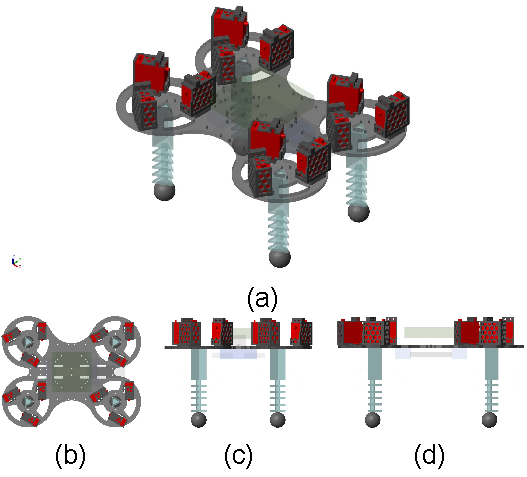
\includegraphics[width=0.5\linewidth]{img/chap1/robot3.pdf}
    \caption{Rendered View of the Previous Quadruped Robot Model. (a) Isometric view; (b) Top view; (c) Front view; (d) Left view.}
    \label{fig:robot3}
\end{figure}

In the previous studies\cite{thorapallimuralidharanContinuumActuatorBased2020} completed by the KTH Mechatronics and Embedded Control Systems Unit, tendon-driven soft continuum actuators were implemented in \ac{3D} /\ac{4D} printed structures to operate as legs of quadruped robots. This soft quadruped robot model developed in MATLAB's Simscape environment as demonstrated in Figure \ref{fig:robot3}. Specifically, the tendons are used to transmit the force from motors, while the soft material acts as the core and the rigid disc acts as the tendon guide to form the actuator body. Since soft legs are inherently compliant to the terrain, they have had an increased capability of traversing complicated environments. Based on this soft leg, a soft quadrupedal robot prototype was developed and gait analysis was performed to enable the robot to walk\cite{daneliaStructureGaitOptimizationof2021}, namely SoftQ. A "gait" in the context of robotics refers to the specific pattern or sequence of leg movements and body motions that a robot follows while walking or moving\cite{akhtaruzzamanGaitAnalysisSystems2016}. It is essentially the coordinated sequence of steps and motions that allows a robot to achieve stable and efficient locomotion\cite{xuGaitAnalysisQuadruped2019}.

Modelling for the actuators and legs are quite important for closed loop control, since the robots will benefit from feedback to the closed loop control when interacting with the terrine. Therefore, the KTH team\cite{muralidharanSoftQuadrupedRobot2021} have already investigated the modeling process of a quadruped robot enabled by four tendon-driven continuum actuators on MathWorks Simulink\textsuperscript{\textregistered}. Based on the developed soft robot simulation model, a gait controller was developed by a \ac{RL} algorithm \ac{SAC} recently\cite{jiSynthesizingOptimalGait2022}.

\ac{RL} has shown great potential in studying the control of quadruped robot motion due to its ability to learn complex control policies through trial-and-error interactions with the environment\cite{rechtTourReinforcementLearning2019}. This approach is particularly relevant for soft quadruped robots, as their continuous and deformable morphology poses significant challenges for traditional control methods\cite{zhangEffectiveSoftRobot2017}. Moreover, \ac{RL} enables the robot to learn from experience, allowing it to optimize its behavior based on feedback received from the environment in the form of a reward signal, thereby leading to the development of more efficient and robust control policies that can handle complex and unpredictable environments\cite{jiLearningbasedControl4D2022}. Consequently, \ac{RL} is ideally suited for studying the control of complex systems such as soft quadruped robots, which are challenging to model and control using traditional methods\cite{rechtTourReinforcementLearning2019}. Although various \ac{RL} algorithms have been used to develop policies for quadruped robots\cite{cebeOnlineDynamicTrajectory2021,chignoliOnlineTrajectoryOptimization2021,chignoliRapidReliableQuadruped2022}, challenges remain in developing RL-based gait control strategies. These strategies need to handle the continuous and deformable morphology of the robot while also being computationally efficient\cite{wangEfficientLearningRobust2022}.  Hence, gait control of soft quadruped robots stands as a promising area of research with the potential to advance the field of soft robotics. However, the traditional learning methods suffer from challenges such as high sample complexity\cite{haarnojaSoftActorCriticOffPolicy2018}, instability during training\cite{zhangUnderstandingDeepLearning2021}, and the need for careful tuning of hyperparameters\cite{haarnojaSoftActorCriticAlgorithms2019}. There is a clear need for further research to develop more efficient and effective RL control strategies that can handle the complexity of these robots and enable them to perform tasks in real-world environments\cite{annaswamyAdaptiveControlIntersections2023}. Looking ahead, \ac{RL} is likely to continue being applied for learning dynamic walking gaits for quadruped robots in both simulated and real-world environments. Moreover, \ac{RL} is expected to be utilized for controlling the behavior of quadruped robots in various tasks, including but not limited to obstacle avoidance and terrain adaptation. These applications of \ac{RL} hold great promise for advancing the field of robotics gait control and improving the efficiency and effectiveness of soft quadruped robots in various practical applications.

In short, the core of this thesis lies at the intersection of two rapidly developing research areas, soft-bodied robotics and reinforcement learning. Incorporating \ac{MBRL}, which involves utilizing models of the environment to improve the efficiency of learning, the thesis focuses on developing innovative control strategies using \ac{MBRL} for proficient gait regulation of soft quadruped robots, intending to promote progress in the field and introduce flexible, efficient robotic systems proficient in navigating complex environment autonomously.

\section{Problem Statement}
The research at hand adopts a novel approach by utilizing \ac{MFRL} for the development of innovative control strategies aimed at proficient movement regulation in soft quadruped robots\cite{jiSynthesizingOptimalGait2022}. Previous work has primarily focused on employing model-free reinforcement learning techniques to address challenges in larger state spaces, offering valuable insights into the potential of reinforcement learning for complex robotic systems. However, there remain several uncovered limitations that warrant meticulous consideration for future endeavors in this domain.

A prominent challenge is the significant time inefficiency inherent in training processes. The iterative nature of \ac{MFRL} and complecity of simulation to soft robot can lead to protracted training times, hindering the real-time application of learned strategies\cite{jiSynthesizingOptimalGait2022}. To address this challenge, innovative approaches have been explored. One such solution is the concept of \ac{MBRL}, which offers a promising approach to mitigate the time efficiency problem. MBRL involves the creation of a functional representation of the robot's interaction with its external environment, closely resembling the physical model of the robot's dynamics, and providing precise state updates in an efficient manner \cite{rayModelBasedReinforcementLearning2010}. Within the MBRL framework, the agent learns a surrogate model of past interactions, mapping specific actions to subsequent observations. This model enables the agent to predict the future state of the environment and the potential outcomes of different actions, empowering the agent to plan ahead and make informed decisions, thereby enhancing learning efficiency and task-solving capabilities\cite{polydorosSurveyModelBasedReinforcement2017}. The surrogate model within an MBRL framework is used to simulate the environment and predict the outcomes of different actions, rather than directly interacting with the real
environment. This approach is considered to speed up learning and improve efficiency.

Furthermore, the complex dynamics of high-dimensional state and action spaces pose a formidable obstacle. The intricate interactions between the soft robot's flexible structure and its environment create a complex learning landscape\cite{arulkumaranDeepReinforcementLearning2017}, making exploration and convergence slower. In specific, the input to the \ac{RL} agent consists of state space and action space, and the state space was defined by available sensor measurements, including robot moving velocity in three directions, rotational angle in three directions and normalized contact force on four feet. The action space was defined by motors on the legs, and three motors on each leg. Therefore, the state-action space of the reinforcement learning reaches 22 dimensions, which expands the computational requirements and leads to sparsity in the reward function. As discussed in the background, the state space of the surrogate model consists of state transitions states and reward function states, which will also reach a significant high dimensions. To address this limitation, exploring dimensionality reduction techniques, such as advanced feature extraction methods\cite{polydorosSurveyModelBasedReinforcement2017} or learned representations\cite{wangBenchmarkingModelBasedReinforcement2019}, could offer more concise and effective representations of the state space, thereby enabling quicker and more adaptive learning. 

To address these challenges, this research employs approaches such as pattern-defined reinforcement learning and parameterization. In the previous training\cite{jiSynthesizingOptimalGait2022}, the gait controllers were learnt from actuator-level, but a popular way to design the locomotion controller in rigid quadruped robots is to define certain gait pattern\cite{zhongAnalysisResearchQuadruped2019}. These includes trot, pace, bound, pronk, gallop, etc.\cite{zhongAnalysisResearchQuadruped2019}. Therefore, if the gait controllers could be defined on certain patterns, the gait controllers could be simplified by some certain gaits and some actions could be composed to reduce the state-action space so as to increase the learning efficiency\cite{owakiQuadrupedRobotExhibiting2017}. For instance, the widely adopted trot, known for stability and balance\cite{allenKinematicGaitAnalysis1994}, is chosen to restrict the movement of soft quadruped robots in reinforcement learning. Trotting is characterized by a two-beat diagonal gait, where diagonal pairs of legs move in unison. Specifically, the front left and rear right legs move together, followed by the front right and rear left legs \cite{fletcherTrot2012}. Another method to restrict the state space of the plant model is parameterization, which parameterizing gait phases and control policies based on the abstraction of a quadruped robot\cite{shaoLearningFreeGait2022}, as demonstrated in previous work\cite{jiOmnidirectionalWalkingQuadruped2022}.

In conclusion, the investigation centers on enhancing the control strategies of soft quadruped robots, bridging the gap between learned strategies and real-time application. The research seeks to contribute to the advancement of robotics by addressing the challenges posed by time efficiency and dimensionality while harnessing the potential of reinforcement learning in the context of soft robotic locomotion control. The subsequent section outlines the research questions framed to guide this study's exploration and investigation.
\subsection*{Research Questions}
To elaborate, the problem addressed in this thesis was initially formulated by a set of research questions, which aimed to identify and explore the challenges and opportunities associated with gait control of soft quadruped robots. The following questions were designed to guide the research process and help frame the problem in a meaningful and relevant way.
\begin{enumerate}
    \item \label{rq1}How to restrict the state space or design a surrogate model with high estimation accuracy of soft quadruped robots plant compared to using Simulink Multibody functions? This model could be extracted as a representation of the real system, allowing for efficient and accurate simulations and training. Some methods considered to restrict the state space:
    \begin{enumerate}
        \item Pattern-defined reinforcement learning, it involves selecting a subset of features based on the certain pattern of quadruped robots, i.e. trot.
        \item Parameterization, the higher-level abstractions of the state-action space, it will use phases between gait and real motors to parameterize gaits of quadruped robots.
    \end{enumerate}
    \item \label{rq2}In comparison to model-free \ac{RL}, to what extend can the model-based \ac{RL} approach generate a better \ac{RL} agent and enhance the ability of a soft quadruped robot to walk in terms of stability, walking speed, and cost-of-transport? The enhancement than model-free \ac{RL} is a benchmark of this project. Furthermore, it is important to evaluate the performance of model-based \ac{RL}, and the evaluation of performance of this project focus on the simulation benefices, so what the trade-off is among the learning efficiency, the simulation accuracy and the long-term planning accuracy in order to train an optimal policy for gait control of soft quadruped robot?
\end{enumerate}
The ultimate goal of this thesis was to advance our understanding of gait control for soft quadruped robots and contribute to the development of effective strategies for controlling their motion. This was achieved by addressing a set of research questions, the answers to which are presented in Chapter \ref{chap6}. 

\section{Scope}
The objective of this study is to investigate and improve the learning efficiency associated with the current methods utilized for an optimal gait control of soft quadruped robots. This thesis proposes a \ac{MBRL} approach to improve the learning efficiency and accuracy of optimal gait control while developing resilient and efficient gait control policies that can handle the continuous and deformable morphology of the robot. Moreover, the research seeks endeavors to make a valuable contribution to the development of more efficient and effective \ac{RL} control strategies that can facilitate soft quadruped robots to perform tasks in real-world scenarios. To validate these concepts, practical physical tests are conducted to corroborate the research's practical applicability and effectiveness. Ultimately, this thesis also introduces a new software architecture tailored to the specific requirements of the  soft quadruped robot SoftQ.

\subsection*{Limitations}
The research faces the challenge of the "sim-to-real gap", where simulations may not perfectly replicate real-world conditions. Simulated environments, while controlled, may fail to capture the intricacies of real-world contexts. Consequently, results derived from simulations may not always align with real-world performance. This limitation stems from the potential disparity between simulation outcomes and real-world behaviors, affecting the practical applicability of simulation-based findings. Additionally, the interconnected nature of the robot's legs restricts the variety of gaits that can be explored, limiting the robot's capacity for certain types of locomotion that require individual leg movement. This constraint hampers the exploration of locomotion strategies relevant to real-world scenarios. Thus, controller evaluation primarily focuses on the robot's stability, walking speed, and cost-of-transport, rather than intricate algorithm details.

\subsection*{Delimitation}
This thesis specifically concentrates on addressing challenges related to model-based reinforcement learning for optimal gait control in soft quadruped robots. To provide clarity and focus, specific delimitation bounds the scope of this study:

\begin{enumerate}
    \item Exclusivity to Soft Quadruped Robots: The research exclusively considers soft quadruped robots and does not encompass other robot categories or diverse robotic systems. This deliberate focus ensures an in-depth analysis of challenges specific to soft quadruped robots.
    \item Exclusion of External Factors: External factors like wind, varying terrains, and obstacles are intentionally omitted from consideration. While these factors significantly impact robotic system performance, their exclusion allows for a concentrated exploration of model-based reinforcement learning challenges in gait control.
    \item Assumption of Fixed Hardware Design: The study operates under the assumption that the hardware design of the soft quadruped robot is both fixed and operational. Variations or modifications in hardware design fall outside the scope of this research.
    \item Limitation to Specific Algorithm: The research confines its investigation to a particular model-based reinforcement learning algorithm, namely, \ac{SAC}. Alternative approaches, methodologies, or algorithms for gait control are not explored within this study.
\end{enumerate}
These delimitations establish the boundaries within which this research operates, enabling a focused and comprehensive examination of the selected challenges in the defined context.

\section{Methodology}
In this degree project, a set of methodologies and methods have been employed to address the research questions and achieve the objectives. The methodology employed comprises four main stages, namely data collection and processing, model-based \ac{RL} algorithm development and comparison, evaluation and analysis, and validation. Detailed description of these methodologies and methods will be presented in Chapter \ref{chap3}. 

This research introduces a novel approach by suggesting that we separately train a surrogate model using RL methods. In this new method, the surrogate model is trained independently from the RL agent, separating the learning processes. This innovative strategy aims to make training more efficient. The surrogate model's job is to simulate the robot's environment and predict what will happen when different actions are taken. This approach, used within the MBRL framework, makes learning faster and more efficient.

Firstly, the signals to motors from the typical trot of quadruped robots were extracted by studying the actuation of the soft quadruped robot trot pattern. Subsequently, a model of the soft quadruped robot was obtained and used to generate simulation data using the Simscape model based on the extracted state space. A surrogate model was then designed with high estimation accuracy of the soft quadruped robot plant based on the processed data, which could effectively simulate the dynamics of the system and train an optimal policy for gait control. After that, a model-based reinforcement learning algorithm was developed for gait control of the soft quadruped robot using the extracted features and the reduced state space. The algorithm's performance was evaluated in simulation using metrics such as stability, walking speed, and cost-of-transport, and its design and parameters were iteratively modified to improve its performance. The previous model-free reinforcement learning algorithm's performance was also evaluated and compared using the same metrics. In the next step, the trade-offs between learning efficiency, simulation accuracy, and long-term planning accuracy were evaluated in the context of training an optimal policy for gait control of the soft quadruped robot. The results were analyzed to draw conclusions about the effectiveness of the proposed model-based reinforcement learning approach compared to model-free reinforcement learning. Finally, the proposed approach was validated by implementing the optimal policy on the physical soft quadruped robot and measuring its performance in a real-world setting in terms of walking speed, stability, and cost-of-transport. The physical robot's performance was compared with the simulated results to validate the accuracy of the simulation and the effectiveness of the proposed approach. The graphical representation depicted in the Figure \ref{fig:method} provides a comprehensive outline of this thesis and enumerates the areas of investigation that have been explored.
\tikzstyle{chevron}=[shape=signal, draw, signal from=west, signal to=east,
    align=center, font=\small, minimum height=3em, draw, minimum width=4em, 
    node distance = 0.5em, inner xsep=1em]

\begin{figure}[ht]
    \centering
    \begin{tikzpicture}[auto]
    \node[chevron, start chain=going right](1){Model design};
    \node[chevron, right=0.5em of 1, on chain](2){\ac{MBRL} algorithm \\development};
    \node(3)[chevron, on chain]{Experiments and \\analysis};
    \node(4)[chevron, on chain]{Validation};
    \node[font=\footnotesize, below=0em of 1,text width=4cm]{-Feature extraction\\ -Data collection\\ -Surrogate model training};
    \node[font=\footnotesize, below=0em of 2,text width=4cm]{-Model implementation\\ -\ac{MBRL} algorithm design\\ -Validate \ac{MBRL} algorithm};
    \node[font=\footnotesize, below=0em of 3,text width=4cm]{-\ac{MFRL} algorithm test\\ -Experiments\\ -Analysis};
    \node[font=\footnotesize, below=0em of 4,text width=4cm]{-Validation on real robot\\ -Evaluation of performance};
    \end{tikzpicture}
    \caption{Overview of the methods in this thesis}
    \label{fig:method}
\end{figure}
 
\section{Ethics and Sustainability}
The use of robotics and artificial intelligence raises ethical and sustainability considerations that need to be addressed in this project. One significant ethical consideration revolves around the potential uses of the quadruped robot in fields like search and rescue, where it can play a crucial role in saving lives and aiding in disaster response. By developing an optimal gait controller for soft quadruped robots, this research contributes to the ethical benefit of improving the efficiency and effectiveness of these robots in life-saving scenarios. Furthermore, the project emphasizes the importance of non-military applications and research, ensuring that the quadruped robot's capabilities are channeled toward humanitarian and constructive purposes. This approach aligns with ethical principles, safeguarding privacy and human rights while maximizing the robot's positive impact. 

Sustainability considerations also play a vital role in the project's framework. This encompasses the environmental impact of materials used in constructing the robot, energy consumption during operation, and waste generation. The project actively addresses these sustainability concerns by prioritizing the use of environmentally-friendly materials in robot construction and focusing on energy-efficient design and testing practices. By doing so, the project seeks to minimize its environmental footprint and contribute to the responsible development of robotic technology.

\section{Outline}
This paper is structured into 6 chapters, beginning with an introductory Chapter \ref{chap1} that provides readers with necessary contextual information and a clear overview of this thesis. Chapter \ref{chap2} is dedicated to a comprehensive review of existing literature in the field, with a particular focus on defining key concepts and providing a thorough problem description. This chapter also deals with the design of soft continuum actuator and the design of the basic structure used to train the neural networks and \ac{RL} agent. Chapter \ref{chap3} outlines the research methods utilized to answer the research questions. Chapter \ref{chap4} is devoted to the implementation of detailed design and the experiments conducted for the research questions. Chapter \ref{chap5} presents the results of the experiments, which also includes the major modifications made to the existing \ac{RL} training method for the improvement. Finally, Chapter \ref{chap6} provides a comprehensive summary of the research project and its future prospects.
